\documentclass{article}

\usepackage{comment}
\usepackage[french]{isodate}

\usepackage{graphicx}
\usepackage{siunitx}
\usepackage{paracol}
\usepackage{amsmath}
\usepackage{ amssymb }
\usepackage[utf8]{inputenc}
\usepackage[bookmarks=true]{hyperref}
\usepackage{bookmark}

\usepackage{mathtools,xparse}

\DeclarePairedDelimiter{\abs}{\lvert}{\rvert}
\DeclarePairedDelimiter{\norm}{\lVert}{\rVert}

%Math typeset and settings
\sisetup{output-decimal-marker = {,}}
\newcommand*{\ft}[1]{_\mathrm{#1}} 
\newcommand*{\dd}{\mathop{}\!\mathrm{d}}
\newcommand*{\tran}{^{\mkern-1.5mu\mathsf{T}}}%transpose of matrix


%Math shortcuts
\newcommand{\vout}{v\ft{out}}

\begin{document}
	\begin{titlepage}
		\begin{center}
			\vspace*{1cm}
			\textbf{Math417}\\
			\text{Mathematical Programming}\\
			\vspace{0.5cm}
			Homework III
			
			\vspace{1.5cm}
			
			\textbf{Frédéric Boileau}\\
			\vspace{2cm}
			Prof. 
			Tim Hoheisel
			\vfill
			\today
			\thispagestyle{empty}
		\end{center}
	\end{titlepage}
	
	\clearpage

	
	
	\section{LP standard form}
	
	By simple manipulations we bring the linear program to standard form:\\
	\begin{align*}
		\min \quad -x_1 - 2x_2  - 3(x_3^+ - x_3^-) \quad \text{ s.t. } \quad  -x_1 -x_3^+ + x_3^- +s_1 &= 0\\
		x_1 - x_3^+  + x_3^- + s_2 &= 0\\
		x_1+x_2 &= 1\\
		x_1,x_2,x_3^+,x_3^-,s_1,s_2 &\ge 0  
	\end{align*}
	
	Now we explicitly write down the parameters.
	\begin{align}
		c = (-1,-2,-3,-3) \quad n = 6 \quad m=3 \\[3ex]
		A = \begin{Bmatrix*}
		-1 & 0 & -1 & 1 & 1 & 0\\
		 1 & 0 & -1 & 1 & 1 & 0\\
		 1 & 0 &  0 & 0 & 0 & 0   
		\end{Bmatrix*}
		\qquad b = \begin{Bmatrix}
		0\\
		0\\
		1
		\end{Bmatrix}
	\end{align}
	\clearpage
  \section{LP modelling}
  
  a)\\
  We can formulate this as follows:\\
  \begin{align}
	  \min \quad 5x_1 + 7x_2 + 4x_3 + 8x_4 + 9x_5 + 10x_6 \quad \text{s.t.} \quad x_1 + x_2 &= 11\\
	  x_3 + x_4 &= 10\\
	  x_5 + x_6 &= 9\\
	  x_1 + x_3 + x_5 &= 18\\
	  x_i &\ge 0
  \end{align}
  
  Where the $x_i$ represent the distances traveled. The first constraints are constraints on the number of trucks needed at the terminals respectively whereas the last one restrains the number we can take from A, which by symmetry also restrains the ones from B. 
  In matrix form we have
  \begin{align}
  	\begin{Bmatrix}
  	1 & 1 & 0 & 0 & 0 & 0 \\
  	0 & 0 & 1 & 1 & 0 & 0 \\
  	0 & 0 & 0 & 0 & 1 & 1 \\
  	1 & 0 & 1 & 0 & 1 & 0 
  	\end{Bmatrix}
  	x = 
  	\begin{Bmatrix}
  	11 \\ 10 \\ 9 \\ 18
  	\end{Bmatrix}
  \end{align}
  
  We row reduce the extended matrix to get 
  \begin{equation}
  	\begin{Bmatrix}
  	1 & 0 & 0 & -1 & 0 & -1 & -1 \\
  	0 & 1 & 0 & 1 & 0 & 1 & 12 \\
  	0 & 0 & 1 & 1 & 0 & 0 & 10 \\
  	0 & 0 & 0 & 0 & 1 & 1 & 9 \\
  	\end{Bmatrix}
  \end{equation}
  
  We notice that the free variables in this form are $x_4$ and $x_6$ 
  which we relabel as $\lambda$ and $\mu$ respectively.
  
  We thus know that every vector which satisfies (1) can be written as
  follows
  \begin{align}
  	x = 
  \begin{Bmatrix} -1 \\ 12 \\10 \\0 \\9 \\0   	\end{Bmatrix}
  + \lambda \begin{Bmatrix} 1 \\ -1 \\ -1 \\ 1 \\0 \\ 0   \end{Bmatrix}
  + \mu \begin{Bmatrix}  1 \\ -1 \\ 0 \\ 0 \\ -1  \\1  \end{Bmatrix} \ge 0
  \end{align}
  
   \begin{align}
    \quad 5(\lambda + \mu) + 7(-\lambda - \mu) + 4(-\lambda) + 8\lambda + 9(-\mu)  +10 \mu = 2\lambda - \mu 
   \end{align}
	
	\clearpage
	
	We know plot the constraints in terms with $\lambda$ as the horizontal axis and $\mu$ as the vertical axis. The inequalities defined in (10) will be drawn for the constraints and we take gradient of the objective function from (11). Since the objective function has a positive sign for $\lambda$ and a negative one for $\mu$ we want "minimize" the first and "maximize" the latter. An objective level curve is drawn in a dotted line. The BFS which minimizes the function is seen to be at $\mu = 9$ and $\lambda=0$
	
	\begin{figure}[htpb]
		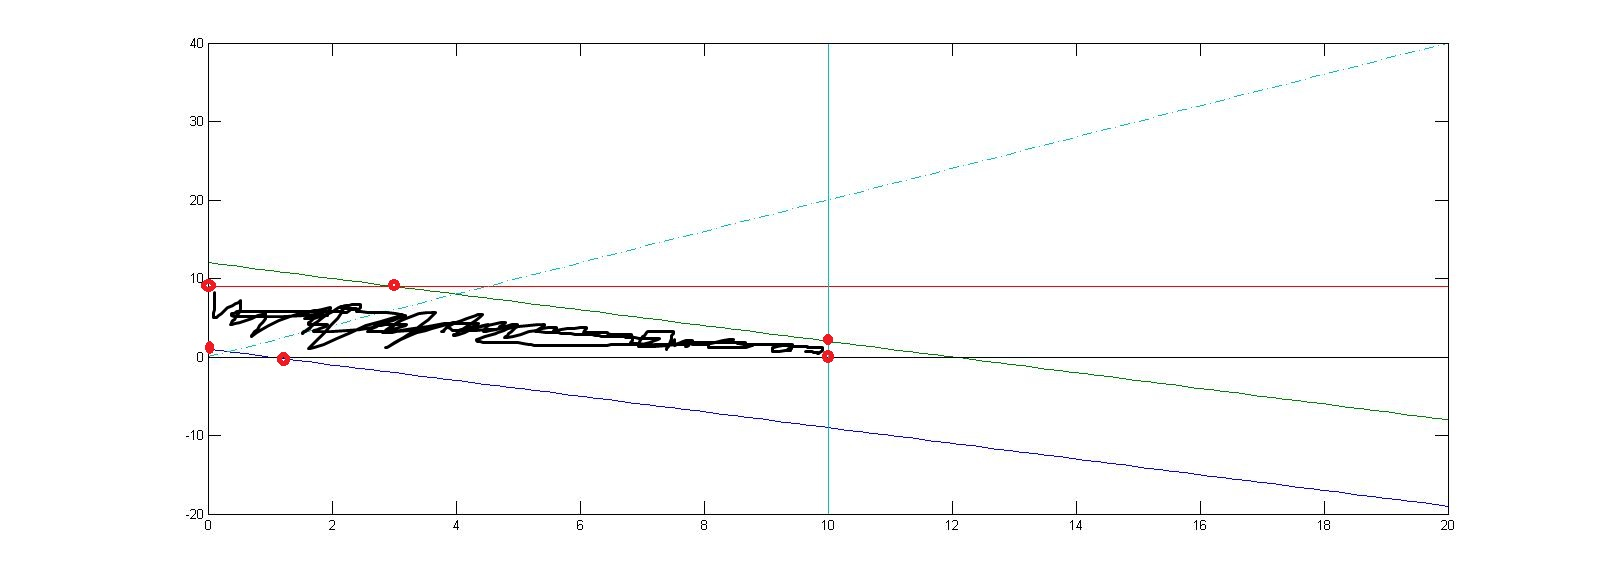
\includegraphics[width = \textwidth]{untitled}
	\end{figure}
	
	 \begin{align}
	 x = 
	 \begin{Bmatrix} 8 \\ 3 \\ 10 \\0 \\0 \\9   	\end{Bmatrix}
	 \end{align}
	 So we have 8 trucks from A to R, 3 trucks from B to R, 10 from A to S and 9 from B to T for a total of 191 km.
	 
	 \clearpage
	 
	 \section{}
	 
	 \begin{align}
	 	f &= \norm{Ax-b}_\infty \\
	 \min f	&= \min \max{\vert a_i\tran x-b \vert }\\
	 \end{align}
	 \begin{align*}
	 	\text{Let } t &= \max \{\vert a_i \tran x - b \vert \}\\
	 	&14 \iff  \min t \text{ but by construction t is defined as s.t.}\\
	 	&\vert a_i\tran x - b_i \vert \le t \times \boldmath{1} \quad \forall \quad i\\
	 	&\iff -t  \times \boldmath{1} \le a_i\tran x - b_i \le t \times \boldmath{1} \quad  \forall \quad i
	 \end{align*}
	 Where the bold 1 is the column vector of length m. The last expression proves a). Now to restate as a standard problem:
	 
	 \begin{align*}
	 	\min \quad t \quad s.t. \quad &t \ge \quad \vert a_i\tran x - b_i \vert\\[3ex] or \quad 
	 	& t \ge a_i\tran x - b_i\\
	 	& t \ge -(a_i\tran x - b_i)\\[3ex]
	 	or \quad & t - s_1 =  a_i\tran x - b_i\\
	 	         & t - s_2 = -(a_i\tran x - b_i)
	 \end{align*}
	 The last constraints being in standard form.
	
	
	
	
	
	
	
	
	
	
\end{document}